\section{Unfolding methods}
\label{sec:UnfoldingMethods}

The migration matrix between truth and reco is used in the traditional unfolding. It is built as a 2D histogram. Unfolding means inferring the generated (truth) from the observed (reconstructed). In Figure~\ref{fig:MigrationMatrix}, the number in a cell represents the probability of an event in the truth bin \emph{i} to be reconstructed in a reco bin \emph{j}. The more diagonalizable matrix, the easier unfolding will be. Events are migrating from one truth bin to other bins for reco, and vice-versa.

\begin{figure}[h]
  \centering
  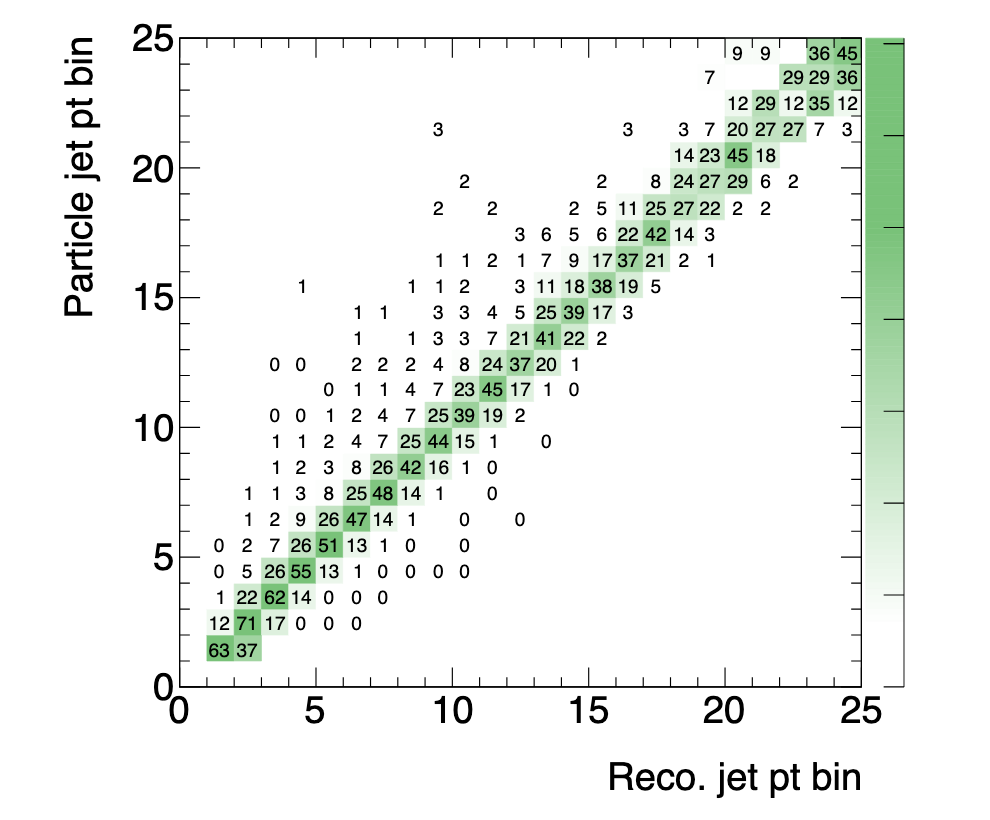
\includegraphics[width=0.98\textwidth]{../presentation/plots/jetPt_migration_matrix.png}
  \caption{The leading particle jet \pt~bin versus the leading reco jet \pt~bin, for the same events of this study~\cite{ReportYichenLi}.}
  \label{fig:MigrationMatrix}
\end{figure}

\ \\A new approach via machine learning has been proposed by A. Glazov at DESY Hamburg~\cite{AGlazov}.

\ \\The two unfolding methods are compared in Figure~\ref{fig:TwoUnfoldingTechniques}. In summary, the traditional method uses binned migration matrix with only one input variable, while the machine learning can learn a continuous function of several input variables.

\begin{figure}[h]
  \centering
  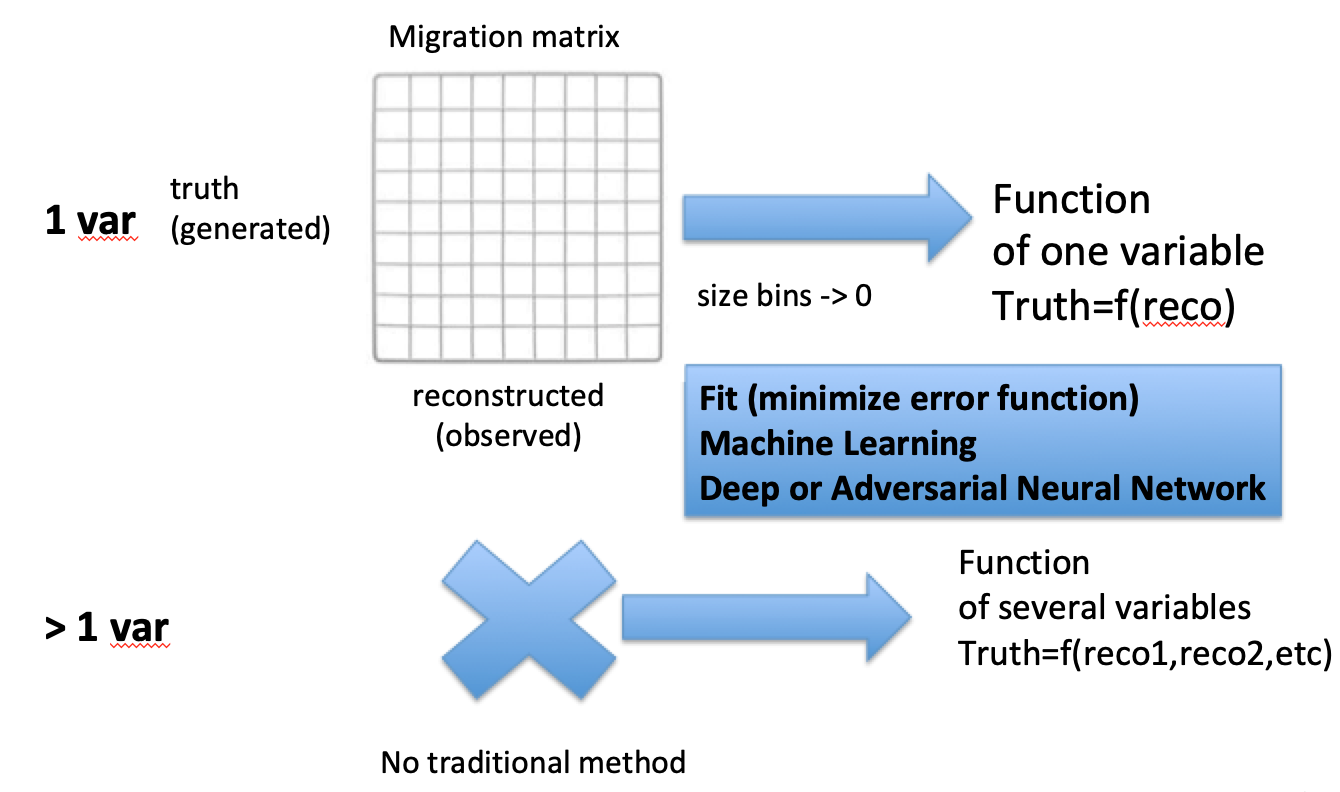
\includegraphics[width=0.98\textwidth]{../presentation/plots/Unfolding_Traditional_ML.png}
  \caption{Comparison of the two unfolding method: traditional (migration matrix, one variable) and machine learning (continuous function, several variables).}
  \label{fig:MigrationMatrix}
\end{figure}
